\section{Hierarchical Agent}
\label{sec:hierarchical_agent}
For the tournament stage of the competition, an agent capable of playing entire matches is needed.
Having previously implemented different agents for each task we can play an entire match alternating between these specific agents.
The difficulty now is to define how to switch between these subpolicies while being competitive against an opponent.

To do so, a high-level agent has been developed. 
This agent decides what policy to execute, based on the observation of the environment and on two main components: the Switcher and the Finite State Machine.

The switcher selects a new policy once the current one has met a termination condition and informed the high level agent.
This new selected policy is selected according to a set of rules applied on the observation state. The switcher's logic is illustrated in Figure \ref{fig:switcher}.
The selected policy could potentially be the previous one. This can happen, for example, if the agent performed a prepare but the
puck is still in an unsuitable position for hitting, a second prepare might be necessary.

The switcher's rules relies on some parameters, therefore it could be trained formulating an optimization problem to find an optimal set of parameters.
To do this we can use PGPE \cite{PGPE}.

Policy Gradients with Parameter-Based Exploration (PGPE) is a reinforcement learning algorithm that enhances exploration by directly perturbing 
the parameters of the policy. Instead of adding noise to the actions at each step, PGPE samples the policy parameters from a distribution, 
leading to a deterministic execution of the policy based on these sampled parameters.
This method is particularly advantageous for optimizing non-differentiable policies, such as the switcher implemented in this work.
Using PGPE, a gaussian distribution $\rho$ over the switcher's parameters $\theta$. 
The algorithm updates the mean $\mu$ and standard deviation $\sigma$ of $\rho$, allowing effective exploration and optimization.

For further details refer to \cite{PGPE}.


% \subsection{Policy gradients with parameter-based exploration}
% PGPE is a policy gradient algorithm that achieves exploration directly perturbing the parameters of the policy. In this formulation, a sample $\theta$ is drawn
% from the parameters distribution $\rho$, and the policy then proceeds deterministically.

% We can formulate an optimization problem defining the performance index

% \begin{equation}
%     \label{eq:pgpe_index}
%     J(\rho) = \int_\Theta \int_H p(h,\theta|\rho)r(h)dh\,d\theta,
% \end{equation}
% where $\theta \in \Theta$ is a parameter vector, $h = [s_{1:T},a_{1:T}] \in H$ is a trajectory, $r(h)=\sum_{t=1}^T r_t$ is the cumulative reward and $rho$ is
% a probability distribution over the parameters $\theta$.

% Differentiating equation \eqref{eq:pgpe_index} we obtain
% \begin{equation}
%     \nabla_\rho J(\rho) = \int_\Theta \int_H p p(h|\theta) p(\theta | \rho) \nabla_\rho \log \p(\theta|\rho) r(h) dh\,d\theta.
% \end{equation}.

% Sampling $\theta$ from $p(\theta|\rho)$ and then running the agent to generate $h$ from $p(h|\theta)$ yields the following gradient estimator:

% \begin{equation}
%     \nabla_\rho J(\rho) \sim \frac{1}{N} \sum_{n=1}^N \nabla_\rho \log p(\theta|rho) r(h^n).
% \end{equation}

% Assuming that 



% A Switcher based on some well defined rules was designed for switching between subpolicies.
% Specifically, the switcher selects the supoliciy and draws an action from it until a terminating condition is met, 
% e.g. the agent finished slowing down after hitting the puck. 
% Every action drawn from a selected subpolicy is returned to the environment.
% The switcher's logic is illustrated in Figure \ref{fig:switcher}. It describes the rules to select the subpolicies.
% The FSM is illustrated in Figure \ref{fig:fsm}.
% Each state represents a task while each
% edge is an allowed transition. The agent will always start a match in the \text{Home} state. It
% is possible to remain in the same state but not switching from a task to another without
% passing from the \textit{Home} state, even if the switcher might suggest a transition of such kind.
% and ensures that after every subpolicy terminates it selects the home policy. This forced return
% to the home position helped adhering more to the constraints that could be violated while switchting from a policy to another. Moreover the policies
% trained with SAC performed better if the robot started from the home position as it was the initial state of every episode it was trained on.


\begin{figure}
    \centering
    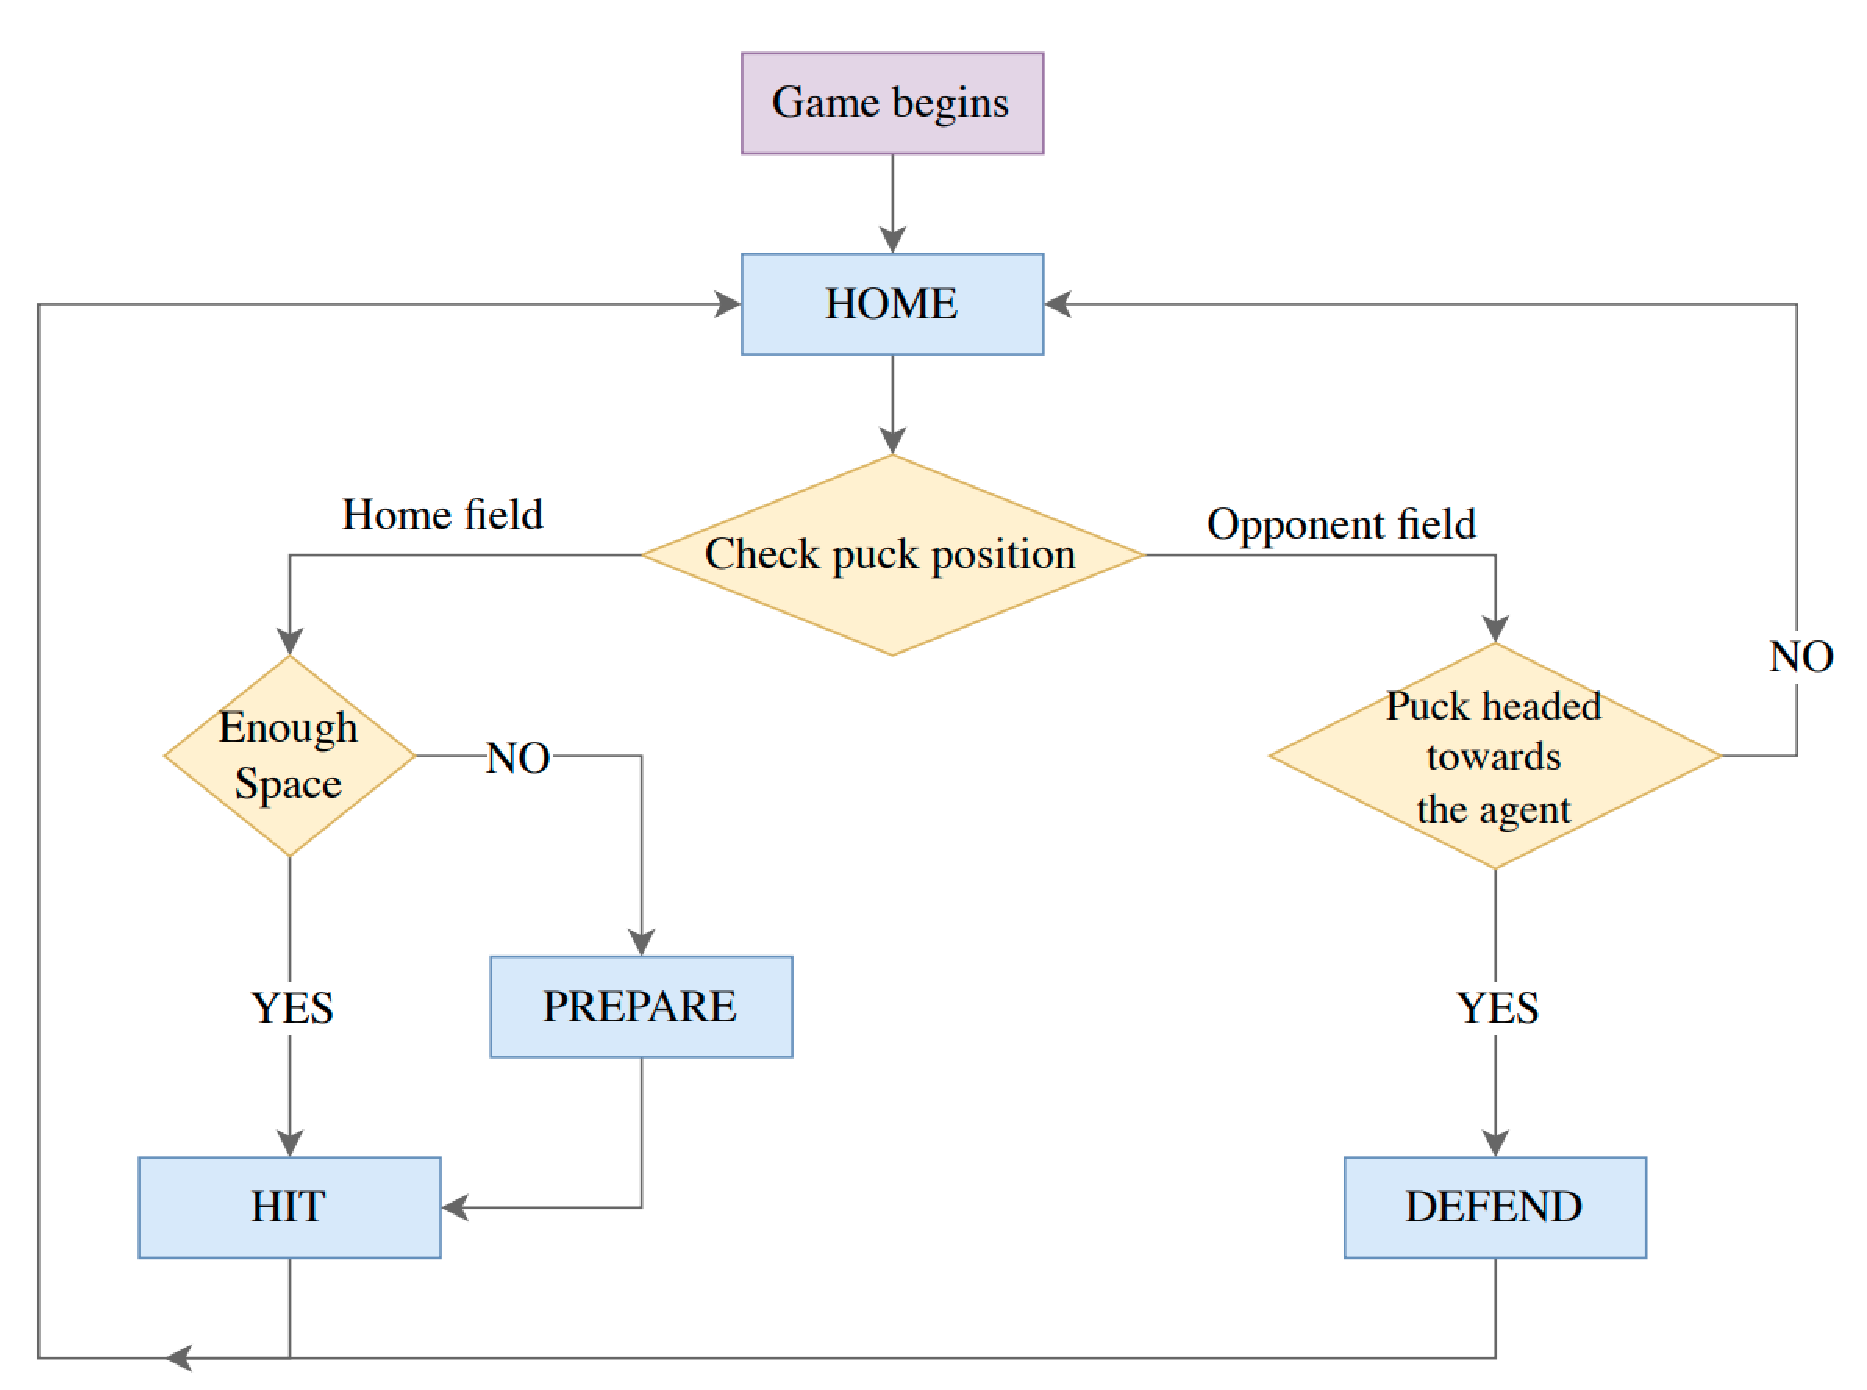
\includegraphics[width=0.9\textwidth]{Images/switcher.pdf}
    \caption{Switcher structure.}
    \label{fig:switcher}
\end{figure}

\begin{figure}
    \centering
    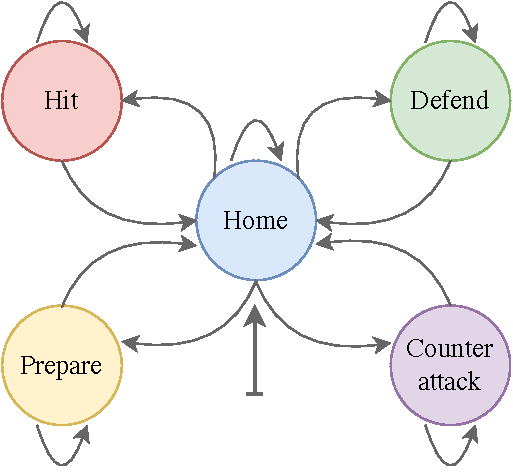
\includegraphics[width=0.5\textwidth]{Images/fsm.pdf}
    \caption{The Finite State Machine.}
    \label{fig:fsm}
\end{figure}